\section{Introduction}
\label{sec.introduction}
As home broadband Internet access is rapidly evolving, broadband networks 
have attracted interests from researchers, policy makers and Internet 
Service Providers (ISPs). The United States alone has more than 279 million 
broadband users and number of Internet users in other regions are even more 
impressive: China has more than 641 million Internet users and other 
developing countries are seeing increased growth~\cite{asia}. Despite their 
pervasiveness, little is known about most home networks hampers progress in 
a number of important research areas, from ISP performance to large-scale 
topology mapping and home network usage. In additional, The intelligent home is now an exciting reality. In 2016, 4 million new "things" will become available to consumers~\cite{gartner}. For these devices to work, they usually need connect to home wireless router. It is possible that hackers are able to open your front door via a buggy software in home wireless router. Therefore, understanding what the vulnerabilities are and preventing these attacks must be considered.

Currently it has been difficult to study home networks on a large scale 
because network technologies like network address translators (NATs) present 
only an opaque view of the home network to the global Internet. To better 
understand home networks, an experimental platform should be hosted in home 
networks, to provide visibility into the missing part of Internet. Such a 
platform also should provide a set of APIs that support the implementation 
of as wide an array of measurement as possible without compromising the 
privacy of the user and abuse of host or network resources. 

Today's measurement and experimentation platform for home networks such as 
BISmark, Samknows and Dasu all support controlled network experimentation 
and broadband characterization. However, the process of vetting BISmark 
experiments is manual, which will be a limiting factor as the deployment 
grows. SamKnows has deployed thousands of home routers in the US and the UK, 
but only supports limited performance measurements. Dasu is a host-based 
software client, thus it is not able to run certain measurements due to 
application restriction and cannot run continuous measurements (i.e., since 
hosts can be turned off, moved, etc.)
 
To address these issues, we developed Seattle Testbed~\cite{seattle}~\cite{zhuang2013experience}~\cite{cappos2009seattle}, an open research and educational testbed that implements a number of measurements primitives that enable researchers, policy makers and Internet Service Providers (ISPs) to program network measurements. Seattle is able to deploy in home wireless router so that it is capable of running both active and passive experiments from a vantage point between the access ISP and the home network, as shown in Fig. 1. To ensure safety, Seattle supports a very flexible language for experiment specification based on Repy which is lightweight, python based, performance isolation and extensible programming language~\cite{cappos2010retaining}. It provides researchers with the ability to install sandboxed measurement applications on the home gateway. 

\begin{figure}%[h]
\centering
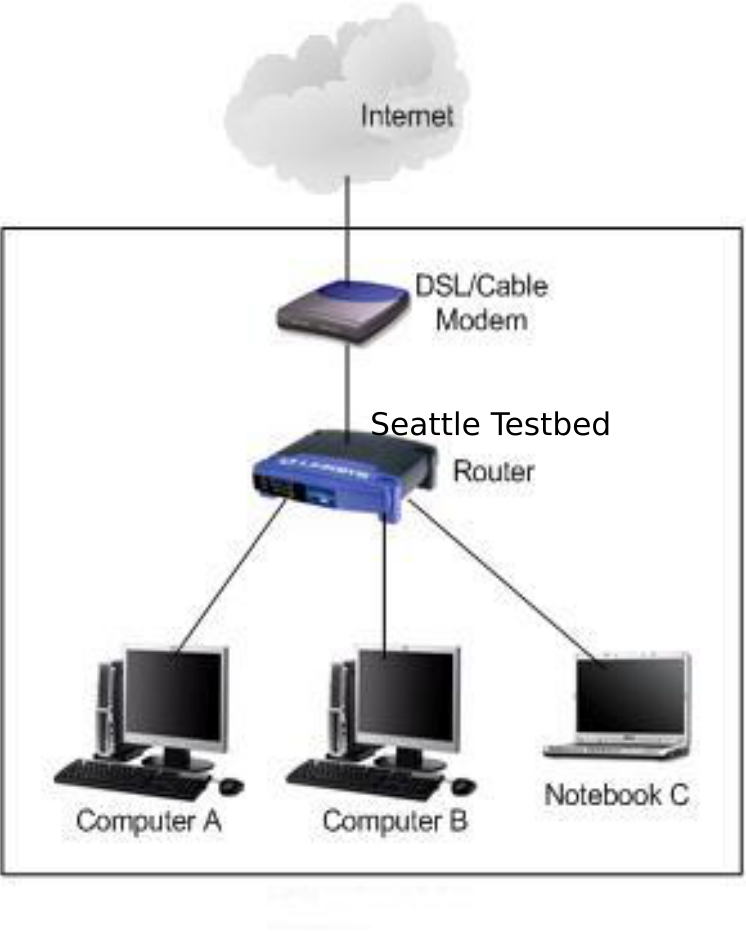
\includegraphics[width=0.5\columnwidth]{figure/home-network.jpg}
\caption{The router sits directly behind the modem in the home network.}
\label{figure:design}
\end{figure}

Both strengths and challenges of a platform like Seattle Testbed stem from 
its inclusion of measurement nodes on the home gateway. First, each nodes 
must be small and easy-to-deploy because Seattle is deployed on resource-
constrained devices. Second, Seattle nodes are on the direct path of real 
Internet users. Thus it must guarantee the safety of the volunteer nodes. 
Third, it is important to make system robustness, remote maintenance and 
update because of the unmanaged complexity of its home network environments. 
Finally, Seattle must provide a rich set of APIs for different network 
measurements.

In this paper, we introduce Seattle Testbed, a distributed cloud platform 
that allows researchers to run their project on system worldwide. This 
testbed provides secure data access while preserving user privacy. Through a 
programmable interface on device, the testbed enables researchers to deploy 
a wide range of network measurements. We also discuss the constraints we 
faced in the design, implementation and deployment of Seattle.
We make the following contributions in this work:
\begin{itemize}
\item\textit{1) Home routers platform:} This platform is based on Seattle\cite{zhuang2013experience}, a community-driven, open-source cloud computing system. Compared to computer and mobile device environments, deployment on home wireless router has more resource limitation such as restricted computational resources. However, recently we are able to port Seattle to embedded devices. Users can build their own Seattle installer (IPK) via config file we provide using OpenWrt SDK and install it on the device directly. 
\item\textit{2) Extensions to Seattle Testbed:}  Our testbed implements new research capabilities for home wireless router by improving on the Seattle sandbox. To handle home wireless routers, our testbed uses low-level system calls in the OpenWrt platform\cite{openwrt} with the Restriction Python (Repy)\cite{cappos2010retaining}, the core sandbox of Seattle. In order to securely interact with home routers on remote user devices, we use Fence~\cite{li2015fence} to allocate a fixed percentage of the device's CPU, memory disk, and other resources to one or more VMs. For example, we set the legal times of accessing proc file system to prevent DoS attack using our API calls. Our testbed adds seven functionalities based on Repy, as shown in in Table I. Through these new functionalities I proposed, researchers are able to implement a wide range of network measurements, as shown in in Table II.
\item\textit{3) Experimental Characterization of home wireless networks: } By integrating Seattle with the home network, we get the benefits of a real world deployment while ensuring flexibility to run experiments without compromising home network. We demonstrate Seattle's utility by implementing one example usage case that together exercise different new API calls (get\_network\_bytes, get\_network\_interface, get\_station): monitoring how busy the WiFi channels in a place over one or two weeks. Our goal is to illustrate how Seattle can support disparate measurement needs.
\end{itemize}